% =====================================================================
% ICIP short paper -- Deterministic Self-Embedding Fragile Watermarking
% Assembled by paper/icip/assemble.py. Edit the part files, not this file.
% Build: tectonic -X compile paper/ICIP_Paper.tex
% =====================================================================
\documentclass[conference]{IEEEtran}
\IEEEoverridecommandlockouts

\usepackage{cite}
\usepackage{amsmath,amssymb}
\usepackage{graphicx}
\usepackage{booktabs}
\usepackage{url}
\usepackage{balance}

\graphicspath{{../output/figures/}{output/figures/}}

\begin{document}

\title{Watermark-Guided Tamper Localization and Recovery: A Key-Seeded
Self-Embedding Fragile Watermarking Scheme with Joint Localization and
Restoration Assessment}

\author{%
\IEEEauthorblockN{Tejas Mane\IEEEauthorrefmark{1}, Shivam Singh\IEEEauthorrefmark{2}, Amol Hipparkar\IEEEauthorrefmark{3}}
\IEEEauthorblockA{Department of Computer Engineering\\
Ajeenkya DY Patil School of Engineering, Pune, India\\
Email: \IEEEauthorrefmark{1}manetejas710@gmail.com,
\IEEEauthorrefmark{2}notshivamsingh@gmail.com,
\IEEEauthorrefmark{3}amolhipparkar04@gmail.com\\
\IEEEauthorrefmark{1}Corresponding author}
\vspace{4pt}\\
\IEEEauthorblockN{Dr.~Deepti Varshney}
\IEEEauthorblockA{Department of Computer Engineering\\
Ajeenkya DY Patil School of Engineering, Pune, India}
}

\maketitle

\begin{abstract}
Passive forensic detectors answer whether an image was edited, but they supply no path back to what the image showed before the edit. This paper presents a deterministic, training-free, key-seeded self-embedding fragile watermark that localizes tampering and restores content jointly. Each $8{\times}8$ block carries, in its two least-significant bit-planes, a 32-bit truncated HMAC-SHA256 tag over its own six most-significant bit-planes and a 96-bit DCT recovery descriptor of a spatially distant partner block selected by a key-seeded single-cycle permutation. A flagged block is rebuilt from the descriptor its surviving partner carries, or explicitly marked unrecoverable. The evaluation covers a 32-image corpus in 3,232 runs over four tamper classes and seven tamper ratios, plus a worked example on an author-supplied $512{\times}512$ photograph. Watermarked images reach 45.48~dB with SSIM 0.9885. Block recall is 1.0000, with block precision structurally forced to 1.0000 by the ground-truth rule, and pixel precision is 0.9599. The recoverability rate $\rho$ stays above its structural bound $1-\alpha$ at every ratio, with mean 0.6482, and in-region recovery reaches 28.49~dB for Variant~A. The scheme is fully fragile, and its one-to-one backup allocation fails all-or-nothing per block, so reference-sharing schemes degrade more gracefully.
\end{abstract}

\begin{IEEEkeywords}
image forensics, fragile watermarking, self-embedding, tamper localization,
content recovery, keyed hash authentication
\end{IEEEkeywords}


\section{Introduction}

Image editing tools are ubiquitous, and convincing manipulation needs no specialist skill. Passive forensic detectors \cite{zhou2018learning,wu2019mantranet} return a probability map of suspected manipulation but offer no path back to the original: the overwritten content is absent from the image they inspect. Active self-embedding \cite{fridrich1999selfembedding,fridrich1999selfcorrecting} places a compressed description of the image inside the image, so the file carries its own repair data and a verifier can ask where it was altered and what the region used to show.

Existing fragile self-embedding schemes break in three recurring ways. First, schemes that authenticate each block independently of its position and of every other block are open to counterfeiting and collage attacks \cite{holliman2000counterfeiting,fridrich2002security}, recombining blocks from different watermarked images into a forgery that still verifies. Second, a block and its backup can fall inside the same tampered region, destroying the repair data with the content it protects; distant block mapping \cite{ausr3} and the tamper-coincidence metrics \cite{tcbr_tcbd} target this failure. Third, evaluations commonly report recovery PSNR without disclosing how much of the tampered area was recoverable, so a high figure can conceal a large unrepaired fraction.

This paper proposes a self-embedding fragile watermarking scheme that is deterministic, training-free, CPU-only and auditable. Every $8{\times}8$ block carries, in its two least-significant bit-planes, a 32-bit truncated HMAC-SHA256 tag over its own six most-significant bit-planes, together with a 96-bit compressed DCT recovery descriptor of a spatially distant partner block. The partner is chosen by a key-seeded single-cycle permutation with an enforced minimum separation, and the tag binds block identity, position and partner descriptor, which defeats block-wise counterfeiting. Verification recomputes each tag; a mismatch localizes tampering at block granularity, and a flagged block is rebuilt from its surviving partner's descriptor or explicitly marked unrecoverable rather than fabricated. Every detection is one recomputed keyed hash comparison, so any third party holding the key obtains the same answer bit for bit, with no training, GPU or run-to-run variance.

The contributions are threefold, and the paper claims nothing beyond them. The first is determinism and auditability: detection is a keyed hash comparison that can be repeated exactly. The second is an explicit keyed construction whose bound fields are each analyzed against the attack they defeat. The third is a joint evaluation of imperceptibility, localization and recovery against exact ground-truth masks, over four tamper classes and seven tamper ratios on a 32-image corpus. The paper does not claim the distant-mapping idea, which belongs to AuSR3 \cite{ausr3}, or superiority over learned proactive schemes, and it reports the recoverability rate and unrecoverable fraction rather than excluding them.

\begin{figure*}[t]
\centering
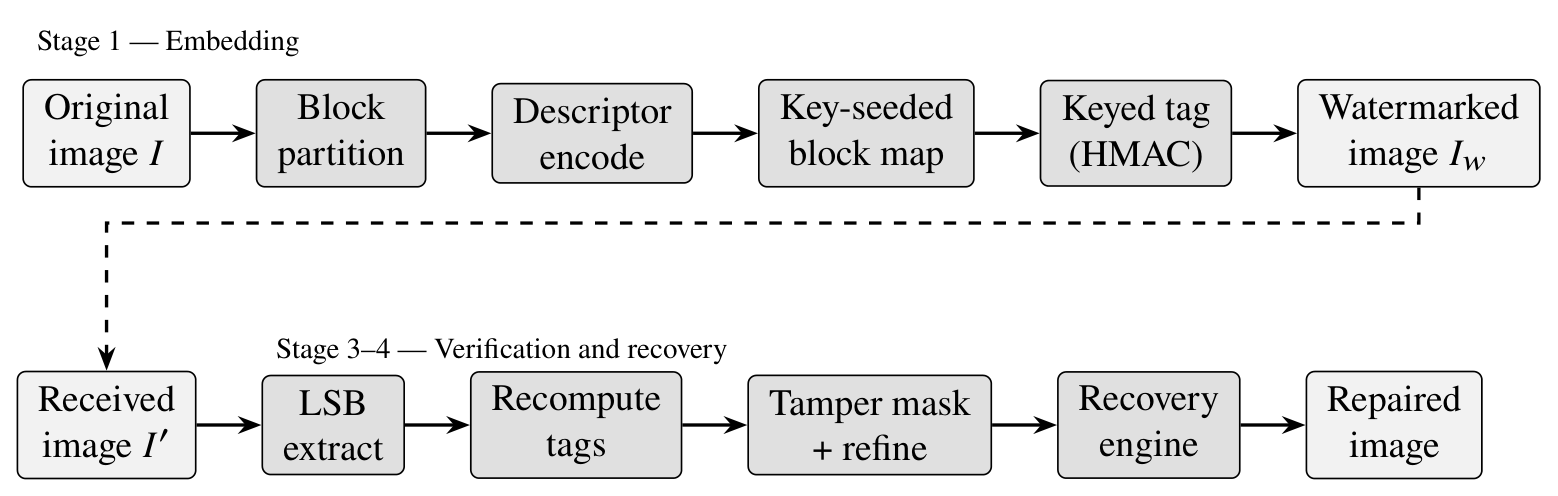
\includegraphics[width=0.88\textwidth]{architecture.png}
\caption{Pipeline. Embedding partitions the image, encodes a recovery descriptor
per block, routes it to a distant partner through the key-seeded map, appends the
keyed tag, and writes both into the two least-significant bit-planes. Verification
recomputes the tag, forms the block mask, and recovers each flagged block from the
descriptor its surviving partner carries.}
\label{fig:arch}
\end{figure*}

\section{Related Work}

\textbf{Fragile authentication and self-embedding.} Fragile watermarking embeds a check value that any modification invalidates. Wong's scheme binds a keyed hash of each block into its least-significant bits \cite{wong2001secret}, and self-embedding \cite{fridrich1999selfembedding} adds a recovery payload so that a damaged block can be rebuilt from data stored elsewhere in the image. Independent per-block checks, however, permit counterfeiting and collage attacks \cite{holliman2000counterfeiting,fridrich2002security}. The accepted fix is keyed binding: each tag covers the block's position and an image identifier, so blocks cannot be transplanted. The present scheme follows that remedy.

\textbf{Recovery-data allocation.} Reference-sharing schemes \cite{zhang2008fragile,zhang2011reference} let several blocks share pooled reference bits, and Korus and Dziech combine reference sharing with fountain-coded allocation \cite{korus2013efficient}. Such allocation degrades gracefully with tampered area, whereas one-to-one allocation fails all-or-nothing for a block whose partner is also damaged. The AuSR family improves the embedding itself through LSB shifting and texture preservation \cite{ausr1}, and AuSR3 introduces distant block mapping to reduce tamper coincidence \cite{ausr3}. The distant-mapping idea is AuSR3's, not a contribution of this paper. The construction here differs in building the map directly in cycle notation from a cryptographically seeded shuffle and in binding the partner descriptor into the tag.

\textbf{Learned and proactive methods.} Passive detectors \cite{zhou2018learning,wu2019mantranet} localize manipulations but do not restore content. EditGuard \cite{editguard} is a learned proactive watermarking method that both localizes and recovers tampered content. This paper does not claim to beat it; the difference is determinism, auditability and the absence of training, not accuracy, since a learned model gives no bit-exact answer that a third party can recompute from a key alone.

The gap addressed is a keyed scheme whose every detection is an auditable hash comparison and whose evaluation reports localization, recovery and the unrecoverable fraction together; existing work either recovers without a bit-exact audit path or audits without stating the recoverable fraction.

\section{Proposed Scheme}
\label{sec:method}

\subsection{Notation and Bit Budget}
\label{ssec:budget}
Each channel of an $M\times N$ image is processed separately and partitioned into non-overlapping $B\times B$ blocks $b_i$, indexed by $i\in\mathcal{K}=\{0,\dots,K-1\}$ in raster order, with $K=\lfloor M/B\rfloor\lfloor N/B\rfloor$. The two least-significant bit-planes of a block hold
\begin{equation}
\mathrm{cap}(B)=2B^{2}\ \text{bits},
\label{eq:cap}
\end{equation}
which is 128~bits per block per channel at $B=8$. This budget splits into a tag of $t$ bits and a recovery descriptor of $d$ bits,
\begin{equation}
t=\min\!\left(32,\ \tfrac{\mathrm{cap}}{2}\right),\qquad d=\mathrm{cap}-t,
\label{eq:split}
\end{equation}
giving $t=32$ and $d=96$ at $B=8$.

The tag cannot cover the embedded planes, which change during embedding. The MSB projection
\begin{equation}
\mathrm{msb}(a)=a\ \mathrm{AND}\ \mathtt{0xFC}
\label{eq:msb}
\end{equation}
zeroes the two low bits of each pixel $a$, is idempotent, and leaves the six high bit-planes untouched. The tag is therefore a function of $\mathrm{msb}(b_i)$ only, written $\mathrm{MSB}(b_i)$ for a whole block.

\subsection{Key-Seeded Block Mapping}
\label{ssec:map}
The scheme stores the recovery descriptor of block $i$ in a spatially distant block $m(i)$, an idea due to \cite{ausr3}; the construction below concerns only key-driven generation. A cryptographically seeded keystream (HMAC-SHA256 in counter mode) drives a Fisher--Yates shuffle of the block indices into an order $\pi=(\pi_0,\dots,\pi_{K-1})$. The map is written directly in cycle notation,
\begin{equation}
m(\pi_t)=\pi_{(t+1)\bmod K},\qquad t=0,\dots,K-1.
\label{eq:cycle}
\end{equation}
For every possible $\pi$, $m$ is a bijection and a single cycle of length $K$, so fixed points, mutual two-cycles and short cycles are absent by construction, not by rejection sampling. With $\mathbf{p}_i$ the centroid of block $i$, the map must also satisfy
\begin{equation}
\lVert\mathbf{p}_i-\mathbf{p}_{m(i)}\rVert_2\ \ge\ d_{\min}=0.25\,\min(M,N)\quad\forall i.
\label{eq:dmin}
\end{equation}
A repair pass swaps elements of $\pi$, keeping a swap only if it strictly reduces the number of violating cycle edges; any rearrangement of $\pi$ still yields a single cycle by (\ref{eq:cycle}), so bijectivity is preserved. The map is regenerated from the key at verification and never transmitted. The separation (\ref{eq:dmin}) ensures that a localized edit destroying block $i$ does not also destroy its backup.

\subsection{Recovery Descriptor}
\label{ssec:desc}
In Variant A, the MSB-projected block is level-shifted by 128 and transformed with an orthonormal 2-D DCT. The first 12 zig-zag coefficients $c_1,\dots,c_{12}$ are retained, each quantized to a signed 8-bit value using the JPEG quality-50 luminance step size $Q_k$ at its position,
\begin{equation}
q_k=\mathrm{clip}\!\left(\mathrm{round}(c_k/Q_k),\,-128,\,127\right),
\label{eq:quant}
\end{equation}
so the descriptor occupies $12\times 8=96$~bits exactly, matching $d$ in (\ref{eq:split}). Decoding dequantizes, inverts the transform, and returns the MSB projection. Variant C is a rate--distortion-fitted adaptive alternative with the same 96~bits.

\subsection{Keyed Authentication Tag}
\label{ssec:tag}
With secret key $K_s$ and image identifier $ID$, the tag of block $i$ is
\begin{equation}
a_i=\mathrm{Trunc}_{32}\!\big(\mathrm{HMAC}_{K_s}(ID\,\Vert\,i\,\Vert\,\mathrm{MSB}(b_i)\,\Vert\,r_{m^{-1}(i)})\big),
\label{eq:tag}
\end{equation}
where $\mathrm{HMAC}$ is HMAC-SHA256 \cite{fips180-4} and $r_{m^{-1}(i)}$ is the 96-bit descriptor that block $i$ physically carries, that of block $m^{-1}(i)$. The implementation also prepends a format tag, geometry, channel and variant code and length-prefixes $ID$ for unambiguous encoding.

Each bound field defeats a specific attack. $ID$ binds the tag to one image, so a block lifted from another image fails. The index $i$ binds position, so swapping blocks or assembling a collage from authentic blocks fails \cite{holliman2000counterfeiting,fridrich2002security}. $\mathrm{MSB}(b_i)$ binds content, so any visible edit of the six high planes fails. The carried descriptor $r_{m^{-1}(i)}$ binds the recovery payload: without it, three quarters of the embedded bits would be unauthenticated, and an attacker could overwrite every descriptor while no block is flagged, so recovery would present forged content as restored. With it, altering a descriptor breaks the tag of the block that carries it. Forging a tag without $K_s$ succeeds with probability $2^{-32}$ per block.

\subsection{Embedding}
\label{ssec:embed}
The descriptor a block carries is computed first, since it depends only on the MSB planes of block $m^{-1}(i)$. Each of a block's 64 pixels carries two payload bits: the first 16 carry the tag and the remaining 48 the descriptor. Descriptor bits are written by LSB \emph{shifting} \cite{ausr1}: a pixel moves to the nearest value whose two low bits equal the target bits, possibly one quantization window away, lowering mean distortion to about 0.5~LSB against about 1.5~LSB for replacement. Tag-carrying pixels are never shifted, since a shift can change their MSB projection and make the tag depend on its own output. The tag is computed over the MSB planes as stored, after the shift.

One map $m$ serves all three channels, each carrying its own tag and descriptor; a per-channel map would make a block recoverable in one channel but not another, producing color-fringed recovery and three unrecoverable masks.

\subsection{Verification and Recovery}
\label{ssec:verify}
The verifier regenerates $m$, extracts the stored tag and descriptor of every block, recomputes (\ref{eq:tag}) over the received MSB planes and the descriptor bits actually present, and compares. A block is flagged if any channel mismatches, yielding the block mask $T$. A light 8-neighbor pass fills unflagged blocks almost fully surrounded by flagged ones; it never clears a flagged block, since an exact keyed comparison yields no false positives to remove. The block mask is expanded to pixels by block replication.

Recovery splits $T$ by backup location. Block $i\in T$ is rebuilt from the descriptor at $m(i)$ if that block verified. The set $U=\{i\in T:\ m(i)\in T\}$ is unrecoverable, as both block and backup were destroyed; these blocks are marked with a fixed value, not fabricated. The recoverability rate is
\begin{equation}
\rho=1-|U|/|T|.
\label{eq:rho}
\end{equation}
For a map independent of the tampered region, a flagged block's partner falls inside the region with probability close to the tampered fraction $\alpha$, so
\begin{equation}
\mathrm{E}[\rho]\approx 1-\alpha.
\label{eq:bound}
\end{equation}
This expectation is structural, depending on region coverage and not on descriptor fidelity.

Cost is one keyed hash and one $B\times B$ transform per block, so embedding and verification are $O(MN)$ without iteration, training or GPU. On a $512\times512\times3$ image, single-threaded Python on a commodity AMD x86-64 CPU measures 473~ms for embedding and 197~ms for verification.

\section{Experimental Setup}
\label{sec:setup}

\textbf{Corpus.} The corpus comprises 32 color images: 8 from the USC-SIPI database \cite{uscsipi} and 24 Kodak images. Every file is pinned by SHA-256, so the corpus reproduces byte for byte. The worked example is the author-supplied $512\times512$ photograph of Fig.~\ref{fig:qual}, center-cropped and Lanczos-resampled from the source capture and stored as PNG before embedding. Because the scheme is fully fragile, the input must be fixed in a lossless container first.

\textbf{Tamper protocol.} Four classes are applied: copy-paste splicing, object removal by inpainting, crop-and-refill, and noise corruption, each at seven nominal ratios $\alpha$ from 0.10 to 0.70 in steps of 0.10. Every class is applied to every image at every ratio and for both descriptor variants. The generator emits an exact ground-truth mask for every trial. On the corpus, the achieved area matches nominal within 0.005 up to $\alpha=0.50$ but reaches only 0.573 and 0.653 at nominal 0.60 and 0.70, so those two rows are nominal only. On the photograph, the achieved area matches nominal within 0.032 at every ratio.

\textbf{Metrics.} Imperceptibility is measured by PSNR and SSIM \cite{wang2004image}. Localization is measured by block- and pixel-level precision and recall against the exact masks. Recovery is measured by the recoverability rate $\rho$ and by in-region recovery PSNR, computed only over the region actually recovered. A block is counted as tampered in the ground truth if the region covers any of its pixels. The two recovery measures are always reported jointly, so that recovery quality can never be read without its coverage.

\textbf{Reproducibility.} The evaluation logs 3,232 runs: a main grid of 1,792 (32 images $\times$ 4 classes $\times$ 7 ratios $\times$ 2 variants), 320 null-condition rows, and 1,120 ablation rows. All seeds are fixed, so every logged row can be regenerated exactly. An automated sanity gate of 27 checks must run before any table or figure is emitted; 25 pass, and 2 soft warnings remain: the inpainting MSB-preserved-miss category, and 3 rows with slightly elevated coincidentally-unchanged pixels.

\begin{table}[t]
\caption{Imperceptibility of the Watermarked Images (Measured, $B=8$, LSB Shifting)}
\label{tab:imperc}
\centering
\begin{tabular}{llcc}
\toprule
Image set & Variant & PSNR (dB) & SSIM \\
\midrule
32-image corpus      & A & 45.479 & 0.98847 \\
32-image corpus      & C & 45.492 & 0.98841 \\
Author photograph    & A & 45.648 & 0.99356 \\
Author photograph    & C & 45.661 & 0.99362 \\
\bottomrule
\end{tabular}
\\[2pt]
\footnotesize The minimum SSIM observed anywhere in the $B=8$ set is 0.97831.
\end{table}

\section{Results and Discussion}
\label{sec:results}

\subsection{Imperceptibility}
Table~\ref{tab:imperc} reports embedding distortion. Over the corpus, Variant A reaches 45.479~dB / SSIM 0.98847 and Variant C reaches 45.492~dB / 0.98841, with a minimum SSIM of 0.97831 over the whole $B=8$ set. On the author-supplied photograph the figures are 45.648~dB / 0.99356 (A) and 45.661~dB / 0.99362 (C). The two variants are practically indistinguishable in distortion, as expected from LSB shifting (about 0.5 LSB on average against about 1.5 for replacement, with tag-carrying pixels never shifted).

\subsection{Localization}
Table~\ref{tab:results} gives localization and recovery. Block recall is 1.0000 for splicing, crop-and-refill and noise, and 0.99998 for inpainting. The shortfall is 17 MSB-preserved-miss blocks in total, the predicted residual of binding the tag to the six MSB planes: a smooth inpainter can reproduce the six MSB planes exactly, and such a block is accepted by construction. Block precision is 1.0000, but this is structurally forced by the ground-truth rule, under which a block counts as tampered if the region covers any of its pixels, and is therefore not evidence of detector quality.

Pixel precision averages 0.9599 and rises from 0.9248 at $\alpha=0.10$ to 0.9797 at $\alpha=0.70$. The shortfall from 1.0 is the $8\times8$ block-quantization penalty, which weighs less as the region grows relative to its boundary; it is not a detector error and cannot shrink without a finer grid. On the photograph, block precision and block recall are both 1.0000 for every class and ratio, with pixel precision 0.9525 on average, from 0.9239 at $\alpha=0.10$ to 0.9752 at $\alpha=0.70$, for the same reason. Neighborhood refinement flagged only 2 blocks out of 10,092,544 verified.

The null condition comprises 320 rows and 1,802,240 block verifications of unmodified watermarked images, with zero false positives and a rule-of-three 95\% upper bound of $1.66\times10^{-6}$. This is a determinism and implementation-consistency check across images, variants and keys, not a measurement of the $2^{-32}$ cryptographic false-accept probability.

\subsection{Recovery}
Across the seven ratios, $\rho$ takes the values 0.9590, 0.8584, 0.7479, 0.6371, 0.5335, 0.4437 and 0.3579 (Fig.~\ref{fig:rho}). It is monotone and near-linear, and sits 3 to 6 percentage points above its structural bound $1-\alpha$ at every ratio. The mean over the main grid is 0.6482. In-region PSNR is 28.49~dB for Variant A and 31.13~dB for Variant C, essentially flat across ratios, whereas whole-image quality falls with coverage. Mapping coverage, not descriptor fidelity, is therefore the dominant constraint on recovery quality: where a partner survives, the block is rebuilt at roughly constant fidelity, and the fraction of blocks with a surviving partner is what decays.

The photograph is a deliberately harder case: its mean $\rho$ is 0.6409 and its in-region PSNR is 23.28~dB (A) and 26.56~dB (C), about 5~dB below the corpus means. It is dominated by high-frequency foliage, which a 12-coefficient DCT descriptor cannot carry, so it is an honest worst-case illustration, not a typical one. Its $\rho$ follows the corpus trajectory, falling from 0.9775 at $\alpha=0.10$ to 0.3154 at $\alpha=0.70$, so the coverage argument holds on a texture-dominated image; only per-block fidelity differs, reflecting descriptor bandwidth, not the mapping.

Figure~\ref{fig:qual} shows a splice at $\alpha=0.30$ with Variant A. Verification flags 1,292 blocks, of which 321 are unrecoverable, giving $\rho=0.7515$. Pixel precision is 0.9522 and in-region PSNR is 23.27~dB. The cyan blocks in the detection panel are marked, not fabricated.

\subsection{Comparison and Ablation}
Table~\ref{tab:compare} sets the measured figures beside published ones, which are cited and not re-implemented. Reference-sharing and fountain-coded schemes \cite{zhang2011reference,korus2013efficient} reach far higher whole-image reconstruction at high damage, for example 37~dB at 50\% damage for the latter. One-to-one allocation gives that up: a flagged block whose single partner is also flagged is lost. Its measured 17.39~dB at 50\% tamper (unmarked convention) is correspondingly lower, and 12.40~dB for the honest marked output. Published recovered qualities of 27.64~dB worst case for AuSR1 \cite{ausr1} and above 30~dB at 50\% tamper for Wu et al.\ \cite{wu2026multifeature} are likewise higher; these come from differing protocols and are not strictly commensurable, while the watermarked fidelity of 45.48~dB is comparable with the 45.57~dB reported for AuSR1. In exchange, it offers determinism, an auditable keyed construction, and disclosure of the unrecoverable fraction.

The block-size ablation, $B=8$ against $B=4$, is an honest trade and not a win. Pixel precision improves from 0.9599 to 0.9794, but in-region PSNR falls from 29.63~dB to 26.78~dB, because the payload drops from 128 to 32 bits per block. The tag halves from 32 to 16 bits, raising the per-block false-accept probability from $2^{-32}$ to $2^{-16}$, about 0.25 expected false accepts on a 16,384-block image. Finer localization is thus bought with weaker authentication and recovery.

\subsection{Limitations}
The scheme is fully fragile: any lossy re-encode, resize or filter destroys the watermark, so it protects images only inside a lossless custody chain. One-to-one allocation fails all-or-nothing per block, and reference sharing degrades more gracefully. Recovery is a low-frequency approximation from 12 DCT coefficients, not the original block. Pixel precision is capped by block quantization, the two highest corpus ratios are nominal only, and at $B=4$ the tag halves to 16 bits. Security rests on key secrecy. No claim of superiority over learned proactive schemes such as EditGuard \cite{editguard} is made.

\begin{figure*}[t]
\centering
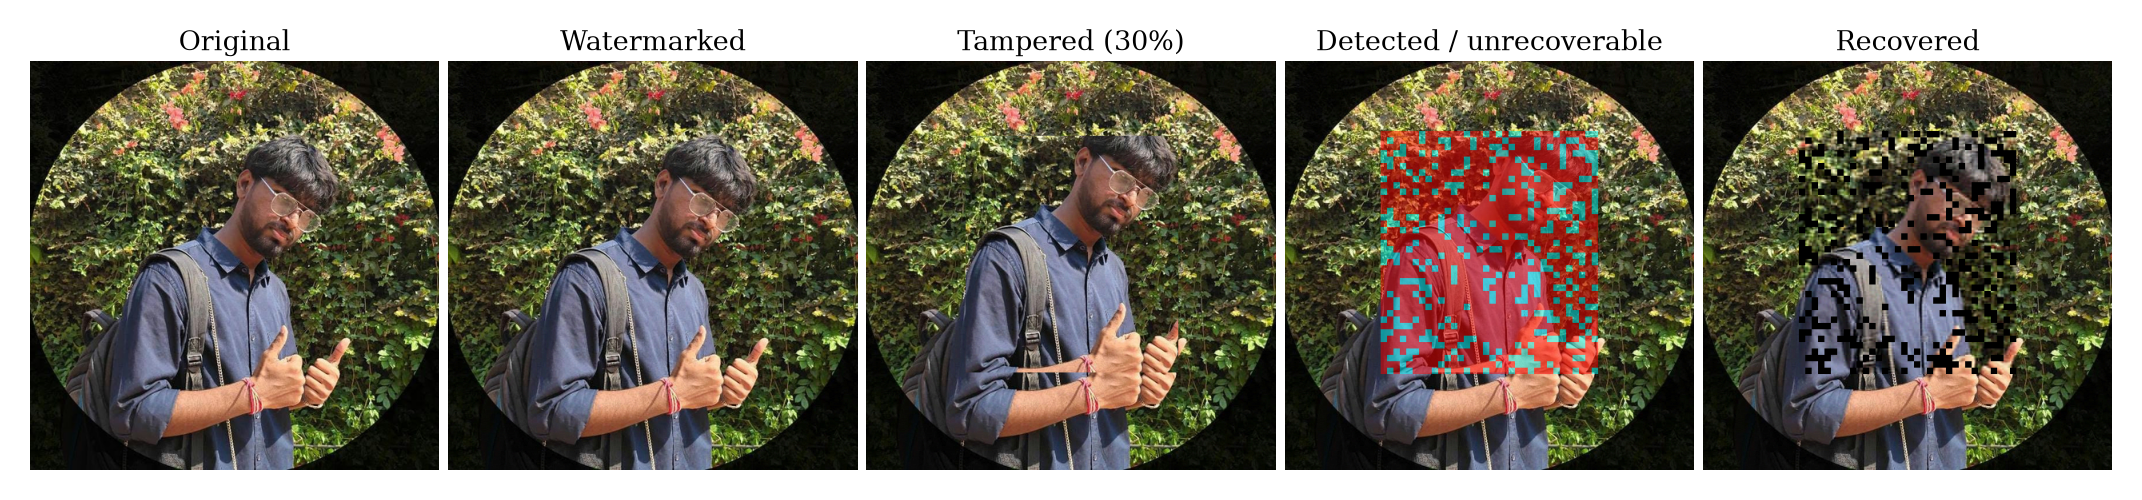
\includegraphics[width=\textwidth]{icip_qualitative.png}
\caption{End-to-end result on the author-supplied $512\times512$ photograph
(copy-paste splicing, $\alpha=0.30$, Variant~A). Left to right: original;
watermarked at 45.648~dB / SSIM 0.99356; tampered; the detected mask, with the
recoverable region in red and the unrecoverable subset $U$ in cyan; and the
recovered image. Of 1{,}292 flagged blocks, 321 fall in $U$ ($\rho=0.7515$) and are
marked black rather than fabricated; pixel precision is 0.9522 and in-region
recovery PSNR 23.27~dB.}
\label{fig:qual}
\end{figure*}

\begin{figure}[t]
\centering
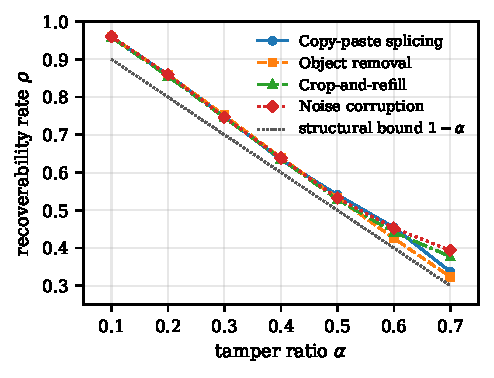
\includegraphics[width=\columnwidth]{icip_rho.pdf}
\caption{Measured recoverability rate $\rho$ against tamper ratio $\alpha$ for the
four tamper classes (Variant~A, $B=8$, 32-image main grid), with the structural
bound $1-\alpha$. The curves sit 3--6 percentage points above the bound at every
ratio and fall monotonically without collapse.}
\label{fig:rho}
\end{figure}

\begin{table}[t]
\caption{Localization and Recovery Against Tamper Ratio. Block-Level Recall Is
1.0000 in Every Row (0.99998 for Inpainting); Block-Level Precision Is 1.0000
Throughout and Is Structurally Forced by the Ground-Truth Rule}
\label{tab:results}
\centering
\begin{tabular}{ccccc}
\toprule
 & \multicolumn{3}{c}{32-image main grid} & Photograph \\
\cmidrule(lr){2-4}\cmidrule(lr){5-5}
$\alpha$ & px.\ prec. & $\rho$ & bound $1-\alpha$ & $\rho$ \\
\midrule
0.10 & 0.9248 & 0.9590 & 0.90 & 0.9775 \\
0.20 & 0.9481 & 0.8584 & 0.80 & 0.8694 \\
0.30 & 0.9581 & 0.7479 & 0.70 & 0.7500 \\
0.40 & 0.9643 & 0.6371 & 0.60 & 0.6356 \\
0.50 & 0.9701 & 0.5335 & 0.50 & 0.5163 \\
0.60 & 0.9740 & 0.4437 & 0.40 & 0.4222 \\
0.70 & 0.9797 & 0.3579 & 0.30 & 0.3154 \\
\midrule
mean & 0.9599 & 0.6482 & --- & 0.6409 \\
\bottomrule
\end{tabular}
\\[2pt]
\footnotesize Corpus rows are means over four tamper classes and both descriptor
variants; the achieved tampered area reaches only 0.573 and 0.653 at nominal 0.60
and 0.70 on the corpus, so those two rows are nominal only.
\end{table}

\begin{table}[t]
\caption{Comparison With Published Self-Embedding Schemes. Figures for Prior Work
Are as Reported by Their Authors and Were Not Re-Implemented Here}
\label{tab:compare}
\centering
\footnotesize
\begin{tabular}{@{}lccc@{}}
\toprule
Scheme & Block & WM PSNR (dB) & Recovered (dB) \\
\midrule
AuSR1 \cite{ausr1}                         & $2\times2$ & 45.57 & 27.64$^{\ast}$ \\
Wu \emph{et al.} \cite{wu2026multifeature} & ---        & $>41$ & $>30$ \\
Korus \& Dziech \cite{korus2013efficient}  & ---        & ---   & 37 \\
This work (Variant A)                      & $8\times8$ & 45.48 & 17.39 \\
\bottomrule
\end{tabular}
\\[2pt]
\footnotesize Recovered PSNR is whole-image at 50\% tamper, except $^{\ast}$AuSR1,
which reports its worst case. The value is convention-dependent: the row for this
work uses the unmarked convention, and the honest marked output is 12.40~dB. This
work additionally reports block recall 1.0000 and pixel precision 0.9599;
Wu \emph{et al.} report 0\% FPR and FNR.
\end{table}

\section{Conclusion and Future Work}
\label{sec:conclusion}

This paper presents a deterministic, training-free, key-seeded self-embedding fragile watermark that localizes tampering at block granularity and rebuilds flagged blocks from a distant partner, or marks them unrecoverable. At 45.479~dB and SSIM 0.98847 on the corpus, the embedding is imperceptible. Block recall is 1.0000 for three of four tamper classes, and the recoverability rate $\rho$ tracks its structural bound with no collapse. Embedding takes 473~ms and verification 197~ms on a $512\times512$ color image, single-threaded and without a GPU. The unrecoverable fraction is disclosed rather than excluded, and the weaker in-region quality on the foliage-dominated photograph is reported as such.

The highest-value upgrade is named directly by the finding that mapping coverage dominates recovery quality: reference sharing or fountain-coded allocation \cite{zhang2011reference,korus2013efficient} would raise coverage without enlarging the descriptor. Further directions are a semi-fragile mode tolerant of benign JPEG re-encoding \cite{linchang2000}, hierarchical localization grids that avoid paying the full tag cost at every level, and integration into capture firmware and PACS ingest.

\balance

\begin{thebibliography}{19}

\bibitem{zhou2018learning} P. Zhou, X. Han, V. I. Morariu, and L. S. Davis, ``Learning rich features for image manipulation detection,'' in \emph{Proc. IEEE/CVF Conf. Computer Vision and Pattern Recognition (CVPR)}, Salt Lake City, UT, USA, Jun. 2018.

\bibitem{wu2019mantranet} Y. Wu, W. AbdAlmageed, and P. Natarajan, ``ManTra-Net: Manipulation tracing network for detection and localization of image forgeries with anomalous features,'' in \emph{Proc. IEEE/CVF Conf. Computer Vision and Pattern Recognition (CVPR)}, Long Beach, CA, USA, Jun. 2019.

\bibitem{fridrich1999selfembedding} J. Fridrich and M. Goljan, ``Protection of digital images using self-embedding,'' in \emph{Proc. Symp. Content Security and Data Hiding in Digital Media}, Newark, NJ, USA, May 1999.

\bibitem{fridrich1999selfcorrecting} J. Fridrich and M. Goljan, ``Images with self-correcting capabilities,'' in \emph{Proc. IEEE Int. Conf. Image Process. (ICIP)}, vol. 3, Kobe, Japan, Oct. 1999, pp. 792--796.

\bibitem{holliman2000counterfeiting} M. Holliman and N. Memon, ``Counterfeiting attacks on oblivious block-wise independent invisible watermarking schemes,'' \emph{IEEE Trans. Image Process.}, vol. 9, no. 3, pp. 432--441, Mar. 2000. DOI: 10.1109/83.826780

\bibitem{fridrich2002security} J. Fridrich, ``Security of fragile authentication watermarks with localization,'' in \emph{Proc. SPIE 4675, Security and Watermarking of Multimedia Contents IV}, San Jose, CA, USA, Jan. 2002, pp. 691--700. DOI: 10.1117/12.465330

\bibitem{ausr3} A. Aminuddin and F. Ernawan, ``AuSR3: A new block mapping technique for image authentication and self-recovery to avoid the tamper coincidence problem,'' \emph{J. King Saud Univ. -- Comput. Inf. Sci.}, vol. 35, no. 9, art. 101755, 2023.

\bibitem{tcbr_tcbd} A. Aminuddin, F. Ernawan, D. Nincarean, A. Amrullah, and D. Ariatmanto, ``TCBR and TCBD: Evaluation metrics for tamper coincidence problem in fragile image watermarking,'' \emph{Eng. Sci. Technol. -- Int. J.}, vol. 56, art. 101790, 2024.

\bibitem{wong2001secret} P. W. Wong and N. Memon, ``Secret and public key image watermarking schemes for image authentication and ownership verification,'' \emph{IEEE Trans. Image Process.}, vol. 10, no. 10, pp. 1593--1601, Oct. 2001.

\bibitem{zhang2008fragile} X. Zhang and S. Wang, ``Fragile watermarking with error-free restoration capability,'' \emph{IEEE Trans. Multimedia}, vol. 10, no. 8, pp. 1490--1499, Dec. 2008.

\bibitem{zhang2011reference} X. Zhang, S. Wang, Z. Qian, and G. Feng, ``Reference sharing mechanism for watermark self-embedding,'' \emph{IEEE Trans. Image Process.}, vol. 20, no. 2, pp. 485--495, Feb. 2011.

\bibitem{korus2013efficient} P. Korus and A. Dziech, ``Efficient method for content reconstruction with self-embedding,'' \emph{IEEE Trans. Image Process.}, vol. 22, no. 3, pp. 1134--1147, Mar. 2013. DOI: 10.1109/TIP.2012.2227769

\bibitem{ausr1} A. Aminuddin and F. Ernawan, ``AuSR1: Authentication and self-recovery using a new image inpainting technique with LSB shifting in fragile image watermarking,'' \emph{J. King Saud Univ. -- Comput. Inf. Sci.}, 2022. DOI: 10.1016/j.jksuci.2022.02.004

\bibitem{editguard} X. Zhang, R. Li, J. Yu, Y. Xu, W. Li, and J. Zhang, ``EditGuard: Versatile image watermarking for tamper localization and copyright protection,'' in \emph{Proc. IEEE/CVF Conf. Computer Vision and Pattern Recognition (CVPR)}, 2024. arXiv:2312.08883.

% TODO(verify-authors): author names for this entry were not resolved in RESEARCH-FINDINGS.md; confirm from the publisher record and add before submission.

\bibitem{fips180-4} National Institute of Standards and Technology, ``Secure Hash Standard (SHS),'' FIPS Publication 180-4, Aug. 2015.

\bibitem{uscsipi} University of Southern California, Signal and Image Processing Institute, ``The USC-SIPI Image Database.'' [Online]. Available: \url{https://sipi.usc.edu/database/}

\bibitem{wang2004image} Z. Wang, A. C. Bovik, H. R. Sheikh, and E. P. Simoncelli, ``Image quality assessment: From error visibility to structural similarity,'' \emph{IEEE Trans. Image Process.}, vol. 13, no. 4, pp. 600--612, Apr. 2004.

\bibitem{wu2026multifeature} Q. Wu, H. Li, M. Li, and M. Wang, ``Multi-feature fragile image watermarking algorithm for tampering blind-detection and content self-recovery,'' \emph{Computers, Materials \& Continua}, vol. 86, no. 1, pp. 1--20, 2026, doi: 10.32604/cmc.2025.068220.

\bibitem{linchang2000} C.-Y. Lin and S.-F. Chang, ``Semi-fragile watermarking for authenticating JPEG visual content,'' in \emph{Proc. SPIE 3971, Security and Watermarking of Multimedia Contents II}, 2000, pp. 140--151. DOI: 10.1117/12.384968

\end{thebibliography}

\end{document}
